\documentclass[10pt]{article}
\usepackage[a4paper, margin=2.1cm]{geometry}
\usepackage{amsmath, amssymb}
\usepackage{graphicx}
\usepackage{booktabs}
\usepackage{microtype}
\usepackage[font=small, labelfont=bf]{caption}
\usepackage{xcolor}
\usepackage{enumitem}
\usepackage[section]{placeins}
\usepackage{tikz}
\usetikzlibrary{arrows.meta}
\usepackage[colorlinks=true, linkcolor=blue!50!black, urlcolor=blue!50!black, citecolor=blue!50!black]{hyperref}
\setlist{itemsep=1pt, topsep=3pt}
\graphicspath{{../figures/}}
\newcommand{\repo}{\url{https://github.com/VaibhavSri245/ell409}}

\title{Trees of Small Neural Networks on CIFAR-10 and Cats vs Dogs:\\ Overfitting, Double Descent, Receptive Fields and Compression}
\author{Vaibhav Srivastava\\ ELL409, IIT Delhi}
\date{October 2026}

\begin{document}
\maketitle

\noindent\textbf{Code:} \repo\ (private repository; README lists every command used for the numbers below).

\section*{Summary}
We built binary trees whose routers and leaves are small multilayer perceptrons, fed them features from three kinds of trunk, and studied them on CIFAR-10 and Cats vs Dogs. The main results:
\begin{enumerate}
\item \emph{Overfitting (E1).} All ten trees (depth 3, 0.3M to 1.3M parameters) reached 100\% training accuracy on the full training sets, with or without the routers made hard. Test accuracy was set by the trunk: 59\%/74\% (CIFAR-10/Cats vs Dogs) with random features, 82\%/91\% with frozen ImageNet ResNet-18 features and 85\%/92\% with a CNN trained separately on the task. Routers that read only shallow trunk features cost at most 1.3 points while halving the parameters used per image.
\item \emph{Double descent (E2).} With 2{,}000 training images and the squared loss, test error peaks where the training loss reaches zero, at $P\approx nK=20$k parameters on CIFAR-10, and falls again past it (20\% noise: 46\% best small tree, 67\% at the peak, 51\% at 308k parameters). Over a grid of 40 depth--width combinations the peak follows the line $P\approx nK$, whether the parameters come from more leaves or wider leaves. More data can hurt (sample-wise peak at $n=P/K$). Cross-entropy moves the peak to about 3k parameters; weight decay $10^{-2}$ removes it and gives the best test error of the sweep (32\%).
\item \emph{Receptive fields (E3).} Every node looks at the whole image, at every depth; nodes differ in the image properties they respond to. With ImageNet features the Cats vs Dogs routers ignore the class and sort photographs by setting (cages, blankets, grass, dark fur); with the task-trained CNN, routing becomes more semantic, saliency moves to the object, and synthesised images show object parts.
\item \emph{Minimising size (E4).} A linear classifier on the same features (9.6k / 1.9k parameters) matches the 1.2M-parameter tree; distilled from the tree it is slightly better. Hard routing runs 18\% of the tree per image; 90\% magnitude pruning costs about 1 point; on Cats vs Dogs the tree can be collapsed from 8 to 3 leaves with no loss of accuracy.
\item \emph{Mislabelled images (E5).} The tree does not quarantine them in a few leaves. When leaves are tiny, the routers bend to the wrong labels; when leaves are large, the leaves memorise them locally, and the second descent comes from test images whose nearest training image is correctly labelled.
\end{enumerate}

\section{Model}
\label{sec:model}

\subsection{Tree of small networks}
A tree of depth $D$ has $2^D-1$ internal nodes (\emph{routers}) and $2^D$ leaves. Every node is a small multilayer perceptron (Figure~\ref{fig:arch}).
\begin{itemize}
\item Router $j$ maps router features $z_r$ to one number $g_j(z_r)$ through one hidden layer of width $h_r$, and sends the image left with probability $p_j(x)=\sigma\!\left(g_j(z_r)/T\right)$, where $T$ is a temperature.
\item Leaf $\ell$ maps leaf features $z_\ell$ to $K$ class scores $f_\ell(z_\ell)$ through one hidden layer of width $h$ (width $0$ means a linear map).
\item The probability that image $x$ reaches leaf $\ell$ is the product of the router decisions on its path,
\[
\mu_\ell(x)=\prod_{j\in\mathrm{path}(\ell)} p_j(x)^{[\ell\text{ is left of }j]}\,\bigl(1-p_j(x)\bigr)^{[\ell\text{ is right of }j]},\qquad \sum_\ell \mu_\ell(x)=1 .
\]
\end{itemize}
With \emph{soft routing} the tree predicts $p(y\mid x)=\sum_\ell \mu_\ell(x)\,\mathrm{softmax}(f_\ell)_y$, a hierarchical mixture of experts \cite{jordan1994}. With \emph{hard routing} each router sends the image to its more likely child, so only $D$ routers and one leaf run per image. Hard routing is the $T\to 0$ limit of soft routing; we report both. The routers and leaves are the same kind of object, so any differentiable classifier can sit at a node; here they are MLPs because the assignment asks for small networks.

\begin{figure}[t]
\centering
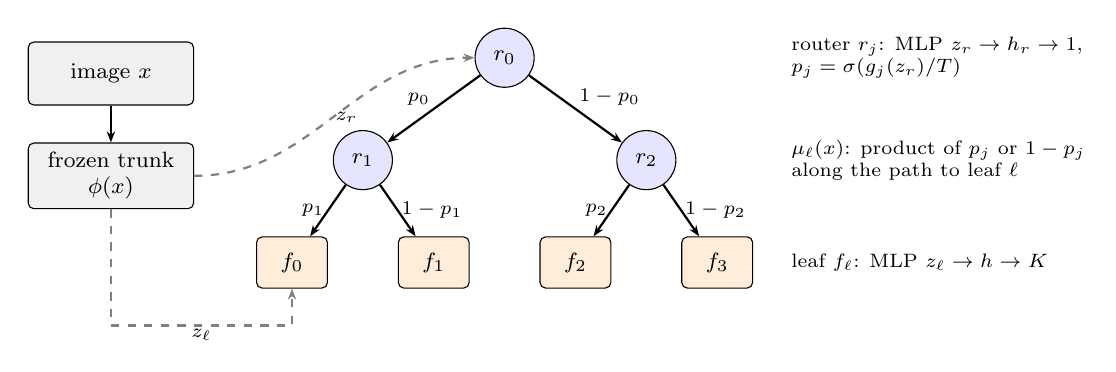
\begin{tikzpicture}[
  font=\footnotesize,
  trunk/.style={draw, rounded corners=2pt, fill=gray!12, minimum width=2.1cm, minimum height=0.8cm, align=center},
  router/.style={draw, circle, fill=blue!10, minimum size=0.75cm, inner sep=0pt},
  leaf/.style={draw, rounded corners=2pt, fill=orange!15, minimum width=0.9cm, minimum height=0.65cm, inner sep=1pt},
  arr/.style={-{Stealth[length=4pt]}, thick},
  lab/.style={font=\scriptsize, inner sep=1pt}]
  \node[trunk] (img) at (0,0) {image $x$};
  \node[trunk] (trk) at (0,-1.3) {frozen trunk\\ $\phi(x)$};
  \draw[arr] (img) -- (trk);
  \node[router] (r0) at (5,0.2) {$r_0$};
  \node[router] (r1) at (3.2,-1.1) {$r_1$};
  \node[router] (r2) at (6.8,-1.1) {$r_2$};
  \node[leaf] (l0) at (2.3,-2.4) {$f_0$};
  \node[leaf] (l1) at (4.1,-2.4) {$f_1$};
  \node[leaf] (l2) at (5.9,-2.4) {$f_2$};
  \node[leaf] (l3) at (7.7,-2.4) {$f_3$};
  \draw[arr] (r0) -- node[lab, above left] {$p_0$} (r1);
  \draw[arr] (r0) -- node[lab, above right] {$1-p_0$} (r2);
  \draw[arr] (r1) -- node[lab, left] {$p_1$} (l0);
  \draw[arr] (r1) -- node[lab, right] {$1-p_1$} (l1);
  \draw[arr] (r2) -- node[lab, left] {$p_2$} (l2);
  \draw[arr] (r2) -- node[lab, right] {$1-p_2$} (l3);
  \draw[arr, dashed, gray] (trk.east) to[out=0, in=180] node[lab, below, black, pos=0.55] {$z_r$} (r0.west);
  \draw[arr, dashed, gray] (trk.south) |- node[lab, below, black, pos=0.75] {$z_\ell$} (2.3,-3.2) -- (l0.south);
  \node[align=left, lab, anchor=west] at (8.6,0.2) {router $r_j$: MLP $z_r \to h_r \to 1$,\\ $p_j = \sigma(g_j(z_r)/T)$};
  \node[align=left, lab, anchor=west] at (8.6,-2.4) {leaf $f_\ell$: MLP $z_\ell \to h \to K$};
  \node[align=left, lab, anchor=west] at (8.6,-1.1) {$\mu_\ell(x)$: product of $p_j$ or $1-p_j$\\ along the path to leaf $\ell$};
\end{tikzpicture}

\caption{The tree used throughout (depth 2 shown). A frozen trunk turns the image into features once; routers read $z_r$ and leaves read $z_\ell$ (every router and every leaf, not only the ones the dashed arrows touch). In \emph{shared} mode $z_r=z_\ell$; in \emph{matched} mode routers read shallow trunk features and leaves read deep ones.}
\label{fig:arch}
\end{figure}

\subsection{Optimisation problem}
This extends the formulation from the previous assignment. With training set $\{(x_i,y_i)\}_{i=1}^n$, router weights $\theta_R$ and leaf weights $\theta_L$, we solve
\begin{equation}
\min_{\theta_R,\theta_L}\;\frac1n\sum_{i=1}^n \mathcal{L}\bigl(y_i;\,\mu(x_i;\theta_R),\,f(x_i;\theta_L)\bigr)\;+\;\beta\,B(\theta_R)\;+\;\lambda\|\theta\|_2^2 ,
\label{eq:obj}
\end{equation}
with two choices of data term:
\begin{align*}
\text{mixture:}\quad &\mathcal{L}=-\log\textstyle\sum_\ell \mu_\ell\,\mathrm{softmax}(f_\ell)_{y} &&\text{(likelihood of the mixture; used for E1, E3, E4)}\\
\text{squared:}\quad &\mathcal{L}=\bigl\|\textstyle\sum_\ell \mu_\ell f_\ell-e_y\bigr\|_2^2 &&\text{(regression on one-hot targets; used for E2, E5)}
\end{align*}
The squared-loss version is also the regression tree asked about in the previous assignment: replace $e_y$ by a real target. $B$ is the balance penalty of Frosst and Hinton \cite{frosst2017}: for each router, $\alpha_j$ is the share of the probability mass reaching it that it sends left, and $B=\sum_j 2^{-\mathrm{level}(j)}\cdot\tfrac12\bigl(-\log\alpha_j-\log(1-\alpha_j)\bigr)$ is smallest when every router splits its traffic evenly. We use $\beta=0.01$ in E1, E3 and E4 and $\beta=0$ in E2 and E5. Weight decay $\lambda$ is $0$ everywhere except the control in Section~\ref{sec:dd}. Everything is trained jointly with Adam (learning rate $10^{-3}$).

\subsection{Implementation}
All routers have the same shape, and so do all leaves, so the $2^D-1$ router MLPs are stored as one stacked tensor of shape $(2^D-1)\times d\times h_r$ and evaluated with a single \texttt{einsum}; the same holds for leaves. A depth-3 tree on 45{,}000 CIFAR-10 feature vectors trains in about 3\,s per epoch on one CPU core. All experiments were run on a 2-core CPU machine with no GPU, which shaped several choices below (cached features, small training subsets for the double-descent sweeps).

\section{Features for the tree}
\label{sec:features}
Raw pixels are a poor input for small MLP nodes: a pixel tree (Section~\ref{sec:rf}) reaches only 48\% test accuracy on CIFAR-10. We therefore give the tree features from a \emph{trunk}, computed once and cached. Three trunks were compared:
\begin{description}
\item[random:] an untrained 3-layer CNN (64--128--256 channels, He initialisation), average-pooled to $2\times2$: 1024 features. It uses no labels and no training.
\item[cnn:] a 4-stage CNN (32--64--128--256 channels) trained separately on the training split for 12 epochs with flips and crops. We keep the pooled stage-2 output (64 features, shallow) and stage-4 output (256 features, deep).
\item[resnet:] ResNet-18 trained on ImageNet \cite{he2016}, used frozen. Images are resized to $64\times64$; we keep the global-average-pooled outputs of all four stages (64+128+256+512 = 960 features). It never sees CIFAR-10 or Cats vs Dogs labels.
\end{description}
Each feature is standardised with training-set mean and variance. Two ways of feeding the tree were compared:
\begin{description}
\item[shared:] every router and leaf reads the full feature vector.
\item[matched:] routers read the \emph{shallow} taps (ResNet stages 1--2, 192 features; CNN stage 2, 64 features) and leaves read the \emph{deep} taps (ResNet stages 3--4, 768 features; CNN stage 4, 256 features). The idea is that a router only needs a coarse cue (colour, texture, layout) to pick a branch, while the leaf has to make the fine decision. This also makes routers cheaper.
\end{description}

\section{Data and protocol}
\begin{itemize}
\item \emph{CIFAR-10}: 45{,}000 training / 5{,}000 validation images (both from the official training set, split with seed 0) and the official 10{,}000 test images, $32\times32$.
\item \emph{Cats vs Dogs}: the Microsoft Asirra set as distributed on Hugging Face (23{,}410 images, label 0 = cat). Images are resized so the short side is 64 and centre-cropped to $64\times64$. Split with seed 0 into 19{,}410 training, 1{,}000 validation and 3{,}000 test images.
\item \emph{Label noise} (E2, E5): a fraction of training labels is replaced by a different, uniformly chosen class, once, before training. Test labels are always clean.
\item \emph{Overfitting runs}: no augmentation, no dropout, no weight decay, no early stopping.
\end{itemize}

\section{E1: fitting the training set}
\label{sec:e1}
Every tree in Table~\ref{tab:e1} is a depth-3 tree (7 routers, 8 leaves) with router width 32 and leaf width 128, trained with the mixture loss, batch size 256, and stopped as soon as training accuracy reached 100\%. All ten runs reached 100\% training accuracy, in 10 to 125 epochs (Figure~\ref{fig:e1}), with no data augmentation and no regularisation other than the small balance term. Hard routing keeps 100\% training accuracy in every case and changes test accuracy by at most 0.5 points, so the routers end up nearly deterministic even though they were trained soft.

\begin{table}[!htbp]
\centering\small
\begin{tabular}{llrrrrrr}
\toprule
dataset & features & params & per image & epochs & train acc & test acc & test acc (hard) \\
\midrule
CIFAR-10 & random, shared & 1290k & 231k & 75 & 100.0 & 59.4 & 59.1 \\
CIFAR-10 & cnn, shared & 411k & 73k & 45 & 100.0 & 85.0 & 84.9 \\
CIFAR-10 & cnn, matched & 288k & 41k & 125 & 100.0 & 84.8 & 84.7 \\
CIFAR-10 & resnet, shared & 1210k & 217k & 20 & 100.0 & 82.5 & 82.1 \\
CIFAR-10 & resnet, matched & 841k & 118k & 30 & 100.0 & 81.1 & 80.7 \\
\midrule
Cats vs Dogs & random, shared & 1281k & 230k & 70 & 100.0 & 73.6 & 73.6 \\
Cats vs Dogs & cnn, shared & 403k & 72k & 75 & 100.0 & 91.7 & 91.6 \\
Cats vs Dogs & cnn, matched & 280k & 39k & 120 & 100.0 & 91.5 & 91.4 \\
Cats vs Dogs & resnet, shared & 1202k & 216k & 10 & 100.0 & 90.6 & 90.6 \\
Cats vs Dogs & resnet, matched & 833k & 117k & 20 & 100.0 & 90.7 & 90.3 \\
\bottomrule
\end{tabular}

\caption{E1. ``per image'' counts the parameters evaluated under hard routing (3 routers and 1 leaf). Test accuracy is with soft routing unless marked hard.}
\label{tab:e1}
\end{table}

\begin{figure}[!htbp]
\centering
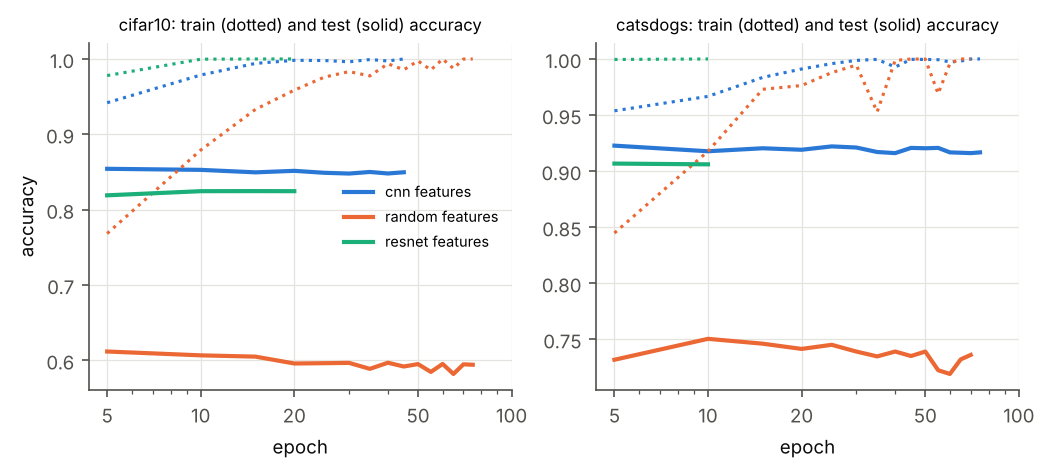
\includegraphics[width=0.92\linewidth]{e1_curves.png}
\caption{E1 training (dotted) and test (solid) accuracy, shared features. Training accuracy reaches 1.0 for every trunk; test accuracy is fixed early and is set by the trunk.}
\label{fig:e1}
\end{figure}

What the table says:
\begin{itemize}
\item \emph{Test accuracy is set by the features.} Random features give 59\% (CIFAR-10) and 74\% (Cats vs Dogs); ImageNet ResNet-18 features give 82\% and 91\%; the CNN trained on the task gives 85\% and 92\%. The tree memorises the training set equally well on all three.
\item \emph{The tree adds nothing on top of a good trunk.} The CNN trunk's own linear head scores 85.8\% (CIFAR-10) and 92.4\% (Cats vs Dogs) on the test set, slightly above the tree trained on its features (85.0\% and 91.7\%). E4 shows the same for ResNet features: a linear classifier matches the 1.2M-parameter tree.
\item \emph{Matched features cost little.} Feeding routers only the shallow ResNet stages (192 numbers instead of 960) cuts the parameters used per image from 217k to 118k and loses 1.3 points on CIFAR-10 and nothing on Cats vs Dogs. With the CNN trunk (routers read 64 shallow features) the per-image count falls from 73k to 41k for a loss of 0.2 points on both datasets. Routers do not need deep features to pick a branch.
\end{itemize}

\section{E3: receptive fields of the nodes}
\label{sec:rf}
For every router of the E1 trees (shared features, ResNet and CNN trunks) we measured:
\begin{enumerate}
\item which classes it sends left and right (test images, hard routing), and the normalised mutual information (NMI) between its decision and the class;
\item its most confident images on each side;
\item its \emph{effective receptive field} \cite{luo2016}: the mean over 64 images that reach the node of $|\partial g_j/\partial x|$, summed over colour channels, with gradients taken through the frozen trunk back to the pixels. The \emph{saliency radius} is the saliency-weighted mean distance from the image centre in units of the half-width; a uniform map gives 0.765 and a map concentrated at the centre gives 0;
\item an image synthesised to push the router hardest each way (gradient ascent on the router score from a grey image, with jitter and a total-variation penalty).
\end{enumerate}
The same saliency is computed for each leaf's score of the true class. We also trained a \emph{pixel tree} (linear routers directly on standardised pixels, leaves with 64 hidden units), whose router weight vectors can be drawn as images. Figures~\ref{fig:rf-cd}--\ref{fig:pixel} show the nodes; Table~\ref{tab:e3sum} summarises them and Tables~\ref{tab:e3-c10}--\ref{tab:e3-cd} list the ResNet routers.

\begin{figure}[p]
\centering
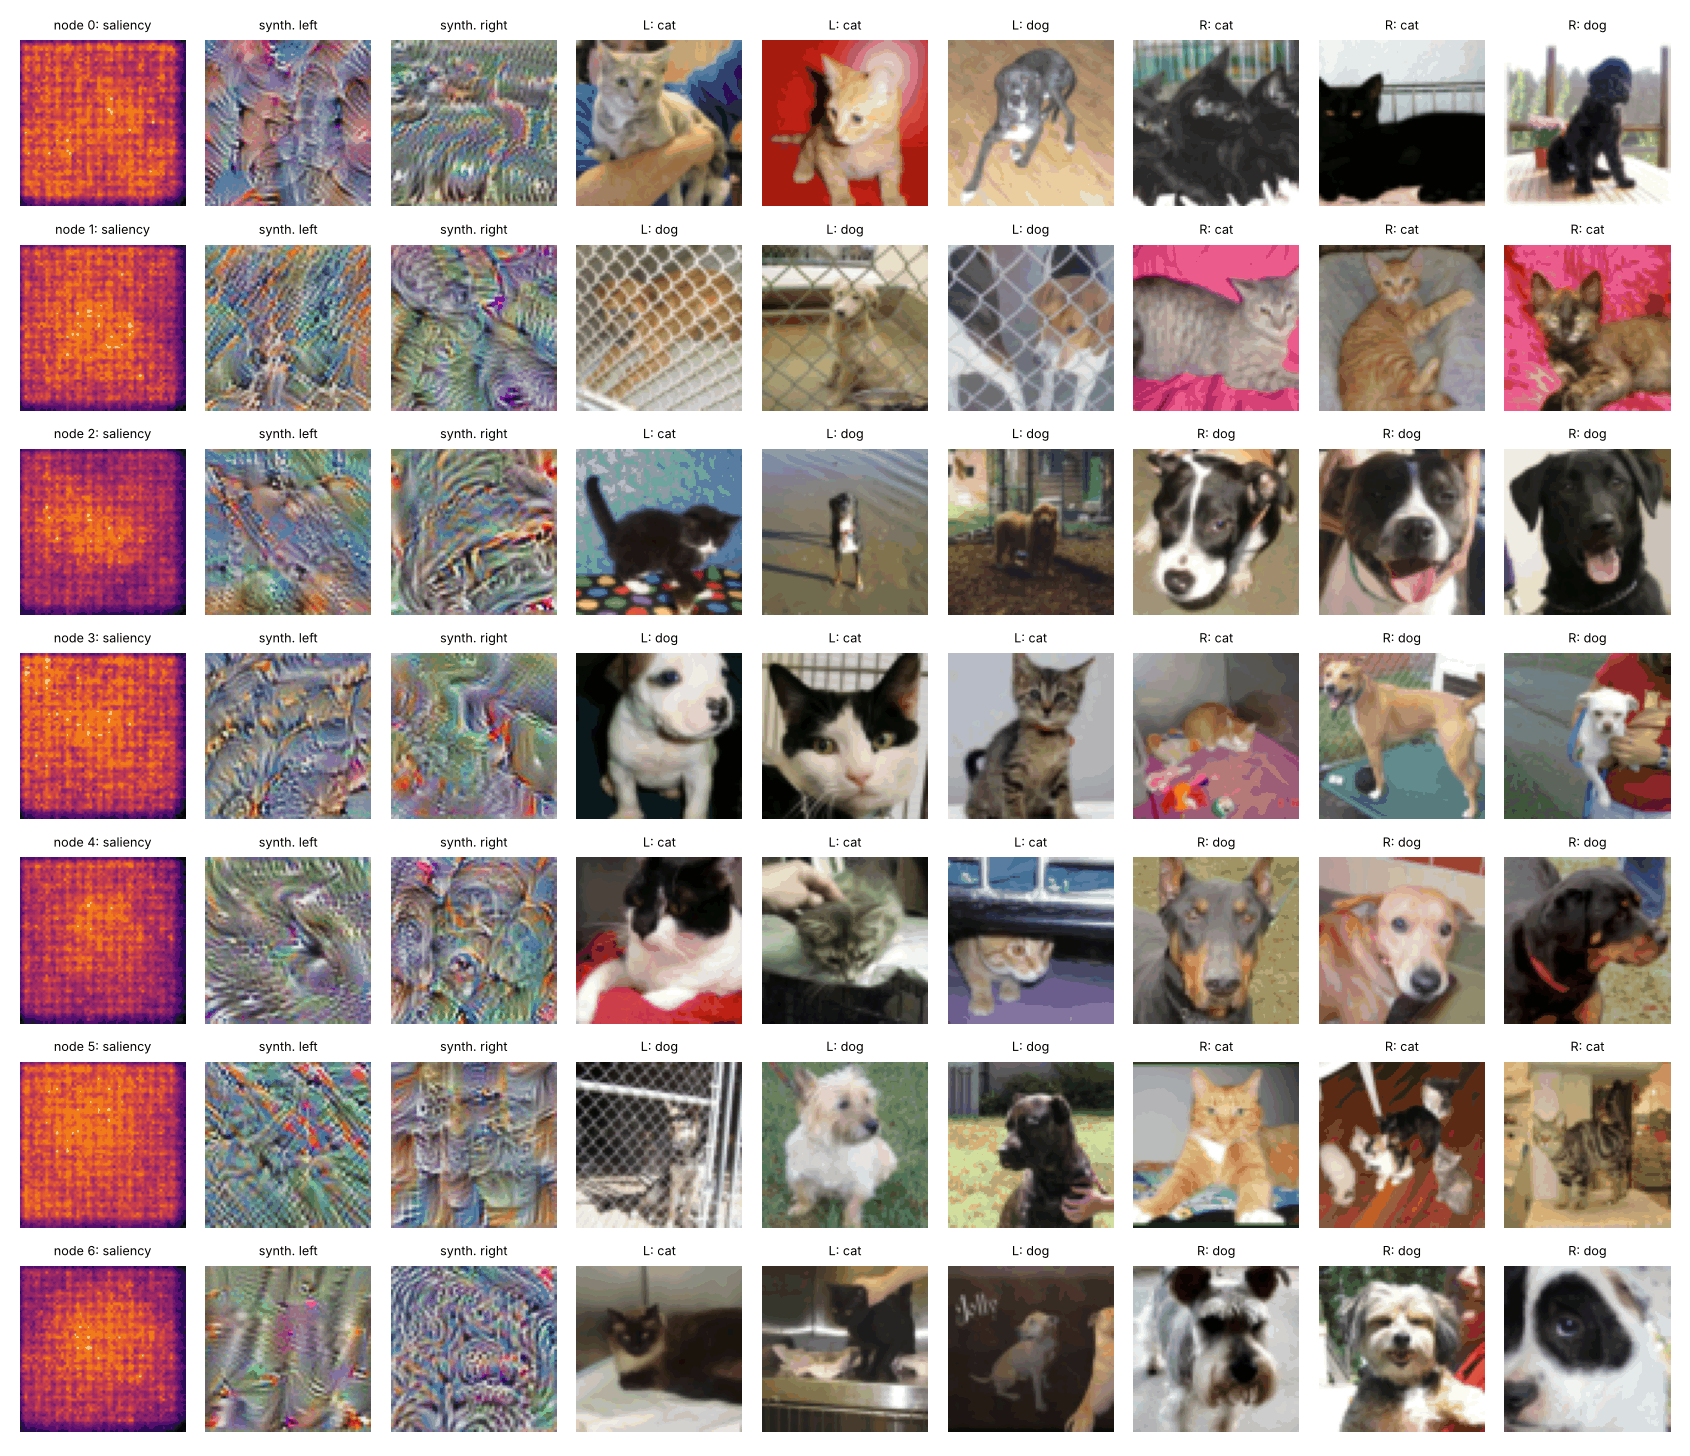
\includegraphics[width=\linewidth]{e3_routers_catsdogs_resnet.png}
\caption{Cats vs Dogs, ResNet features: the 7 routers (rows). Columns: mean input-gradient saliency over images reaching the node; synthesised images pushing the router left and right; the 3 most confident left images; the 3 most confident right images. Node 1 separates dogs behind wire fences and in cages from cats on pink and soft blankets; node 0 sends dark animals right; node 2 separates full-body shots on the ground from close-up dog faces.}
\label{fig:rf-cd}
\end{figure}

\begin{figure}[p]
\centering
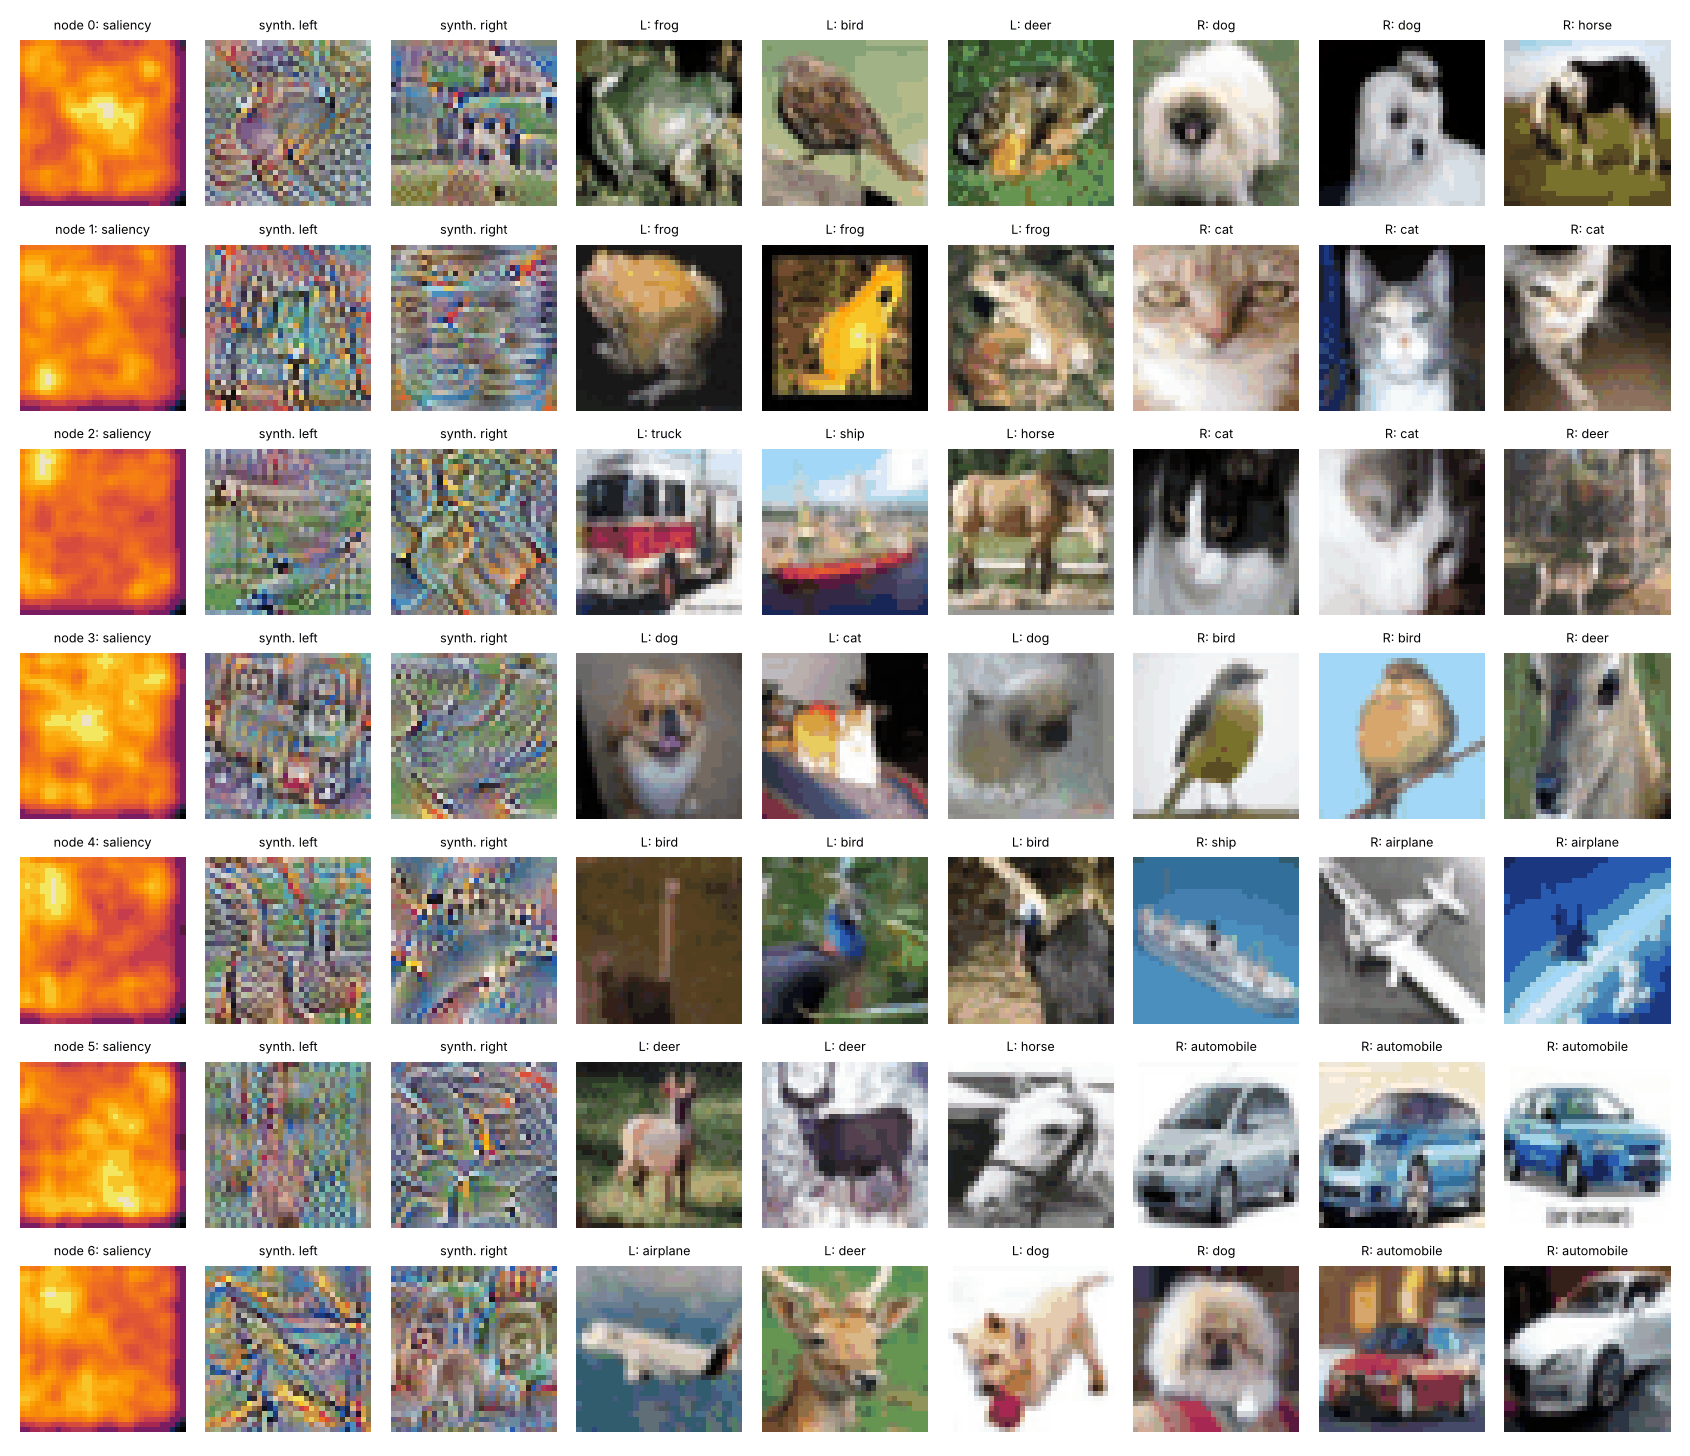
\includegraphics[width=\linewidth]{e3_routers_cifar10_resnet.png}
\caption{CIFAR-10, ResNet (ImageNet) features, same layout. Saliency is spread over the whole image and the synthesised images are textures. Node 4 sends birds in foliage left and ships and aeroplanes on blue backgrounds right; node 5 sends deer and horses left and cars right.}
\label{fig:rf-c10}
\end{figure}

\begin{figure}[p]
\centering
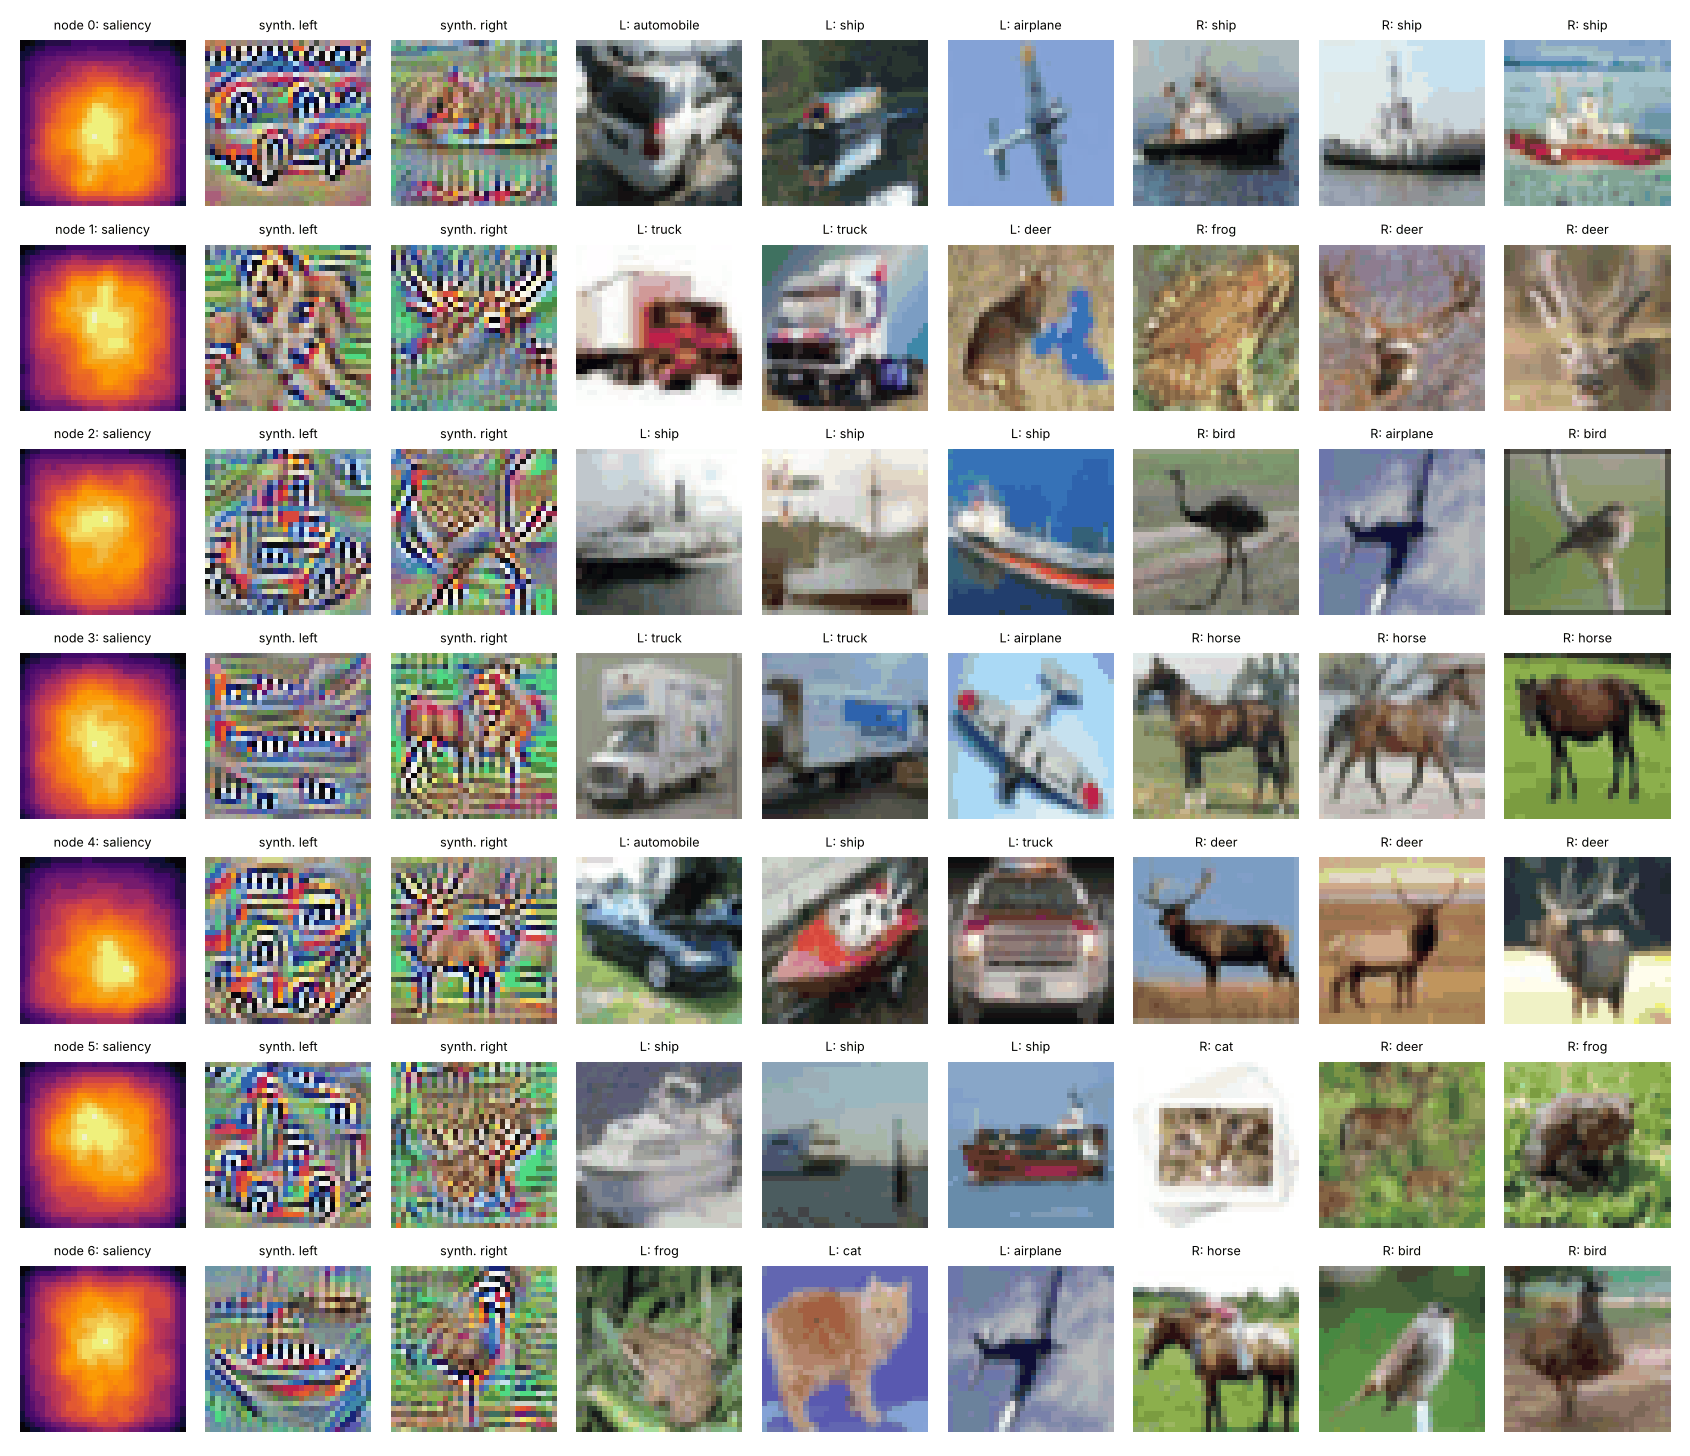
\includegraphics[width=\linewidth]{e3_routers_cifar10_cnn.png}
\caption{CIFAR-10, features from the CNN trained on CIFAR-10, same layout. Saliency now sits on the centre of the image, where the object is, and the synthesised images contain object parts: wheels and car bodies (node 0, left), antlers and legs (nodes 1 and 4, right), a horse (node 3, right), a bird (node 6, right). The root sends vehicles left.}
\label{fig:rf-c10-cnn}
\end{figure}

\begin{table}[t]
\centering\small
\begin{tabular}{llrrrrr}
\toprule
dataset & trunk & NMI(leaf, class) & NMI(root, vehicle) & mean router NMI & router radius & leaf radius \\
\midrule
CIFAR-10 & resnet & 0.225 & 0.044 & 0.125 & 0.74--0.76 & 0.74--0.75 \\
CIFAR-10 & cnn & 0.358 & 0.154 & 0.214 & 0.67--0.69 & 0.66--0.67 \\
Cats vs Dogs & resnet & 0.052 & -- & 0.057 & 0.71--0.74 & 0.71--0.74 \\
Cats vs Dogs & cnn & 0.145 & -- & 0.146 & 0.66--0.72 & 0.65--0.70 \\
\bottomrule
\end{tabular}

\caption{Receptive-field summary for the E1 trees. NMI(root, vehicle): agreement of the root decision with the animal/vehicle grouping. Radius: saliency-weighted distance from the centre (uniform map: 0.765).}
\label{tab:e3sum}
\end{table}

\begin{table}[t]
\centering\small
\begin{tabular}{rrlllr}
\toprule
node & images & left: top classes & right: top classes & NMI(split, class) & saliency radius \\
\midrule
0 & 10000 & frog, bird & truck, horse & 0.109 & 0.74 \\
1 & 5217 & frog, bird & cat, ship & 0.092 & 0.75 \\
2 & 4783 & truck, horse & dog, deer & 0.082 & 0.76 \\
3 & 3005 & frog, cat & frog, bird & 0.130 & 0.75 \\
4 & 2212 & cat, bird & ship, airplane & 0.152 & 0.76 \\
5 & 3047 & horse, truck & automobile, truck & 0.179 & 0.75 \\
6 & 1736 & deer, horse & dog, automobile & 0.134 & 0.75 \\
\bottomrule
\end{tabular}

\caption{CIFAR-10 routers, ResNet features.}
\label{tab:e3-c10}
\vspace{6pt}
\begin{tabular}{rrlllr}
\toprule
node & images & left: top classes & right: top classes & NMI(split, class) & saliency radius \\
\midrule
0 & 3000 & dog, cat & cat, dog & 0.003 & 0.74 \\
1 & 1672 & dog, cat & cat, dog & 0.030 & 0.73 \\
2 & 1328 & cat, dog & cat, dog & 0.001 & 0.72 \\
3 & 896 & dog, cat & dog, cat & 0.000 & 0.74 \\
4 & 776 & cat, dog & dog, cat & 0.149 & 0.72 \\
5 & 622 & dog, cat & cat, dog & 0.139 & 0.74 \\
6 & 706 & cat, dog & dog, cat & 0.076 & 0.71 \\
\bottomrule
\end{tabular}

\caption{Cats vs Dogs routers, ResNet features.}
\label{tab:e3-cd}
\end{table}

\paragraph{Observations.}
\begin{itemize}
\item \emph{On Cats vs Dogs the routers do not split by class.} With ResNet features the NMI between each router's decision and the label is between 0.000 and 0.15, and every leaf receives a mix of cats and dogs (NMI between leaf and class 0.05). The routers split by \emph{context}: wire fences and cages versus soft furnishings (node 1), dark versus light animals (node 0), whole body versus close-up face (node 2), grass and outdoors versus indoors (node 5). Each leaf then solves cat versus dog within one context, at 87--96\% test accuracy per leaf. With two classes there is little to route by class, and the balance penalty asks every router for an even split, so the routers follow the next strongest direction of variation in the features: background and photographic setting. These are the cues a classifier could use as shortcuts; here they decide which leaf sees the image rather than the label.
\item \emph{On CIFAR-10 the routers mix semantics and appearance.} With ResNet features the root does not separate animals from vehicles (NMI with that grouping 0.04); it sends frogs, birds and cats one way and trucks, horses and cars the other. The deepest routers are the most class-like (NMI 0.13 to 0.18, against 0.08 to 0.11 above them), and some splits group classes by background colour: node 4 puts ships and aeroplanes (sky and sea) together against birds in foliage.
\item \emph{The trunk decides what the nodes can see.} With the CNN trained on the task, routing is more semantic (leaf--class NMI 0.36 against 0.23 on CIFAR-10; root--vehicle NMI 0.15 against 0.04), saliency moves to the centre (radius 0.66--0.69 against 0.74--0.76) and the synthesised images show object parts instead of textures (Figure~\ref{fig:rf-c10-cnn}). The ImageNet trunk was never asked to find CIFAR objects, and at $64\times64$ its pooled features describe the whole scene; the task-trained trunk has learned to look at the centred object.
\item \emph{Depth in the tree does not shrink the receptive field.} For both trunks, radii of the root, the deeper routers and the leaves are within 0.07 of each other. The trunk ends in global average pooling, so every feature already depends on the whole image; nodes differ in \emph{what} they respond to (colour, texture, background, parts), not \emph{where}. This is unlike a CNN, where deeper units see larger regions: the tree's depth is a depth of decisions, not of spatial processing.
\item \emph{Pixel-tree routers memorise.} The router weights of the pixel tree (Figure~\ref{fig:pixel}) are mostly high-frequency noise; only the low-pass view shows structure (node 4 weights the border, nodes 2 and 5 a central blob). The pixel tree reaches 87\% training accuracy after 30 epochs but only 48\% test accuracy on CIFAR-10 (99\% and 65\% on Cats vs Dogs), which is why the main experiments use trunk features.
\end{itemize}

\begin{figure}[t]
\centering
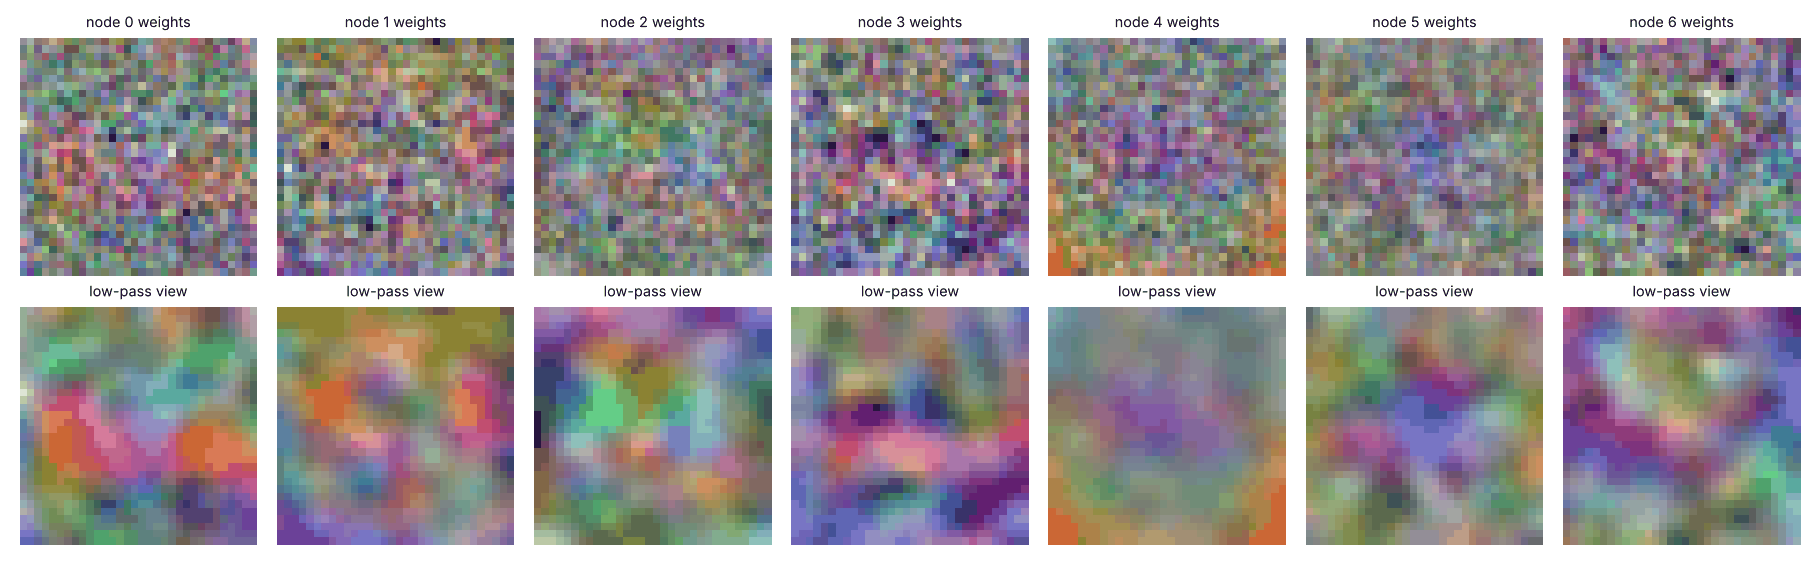
\includegraphics[width=\linewidth]{e3_pixeltree_cifar10.png}
\caption{Pixel tree on CIFAR-10: weights of the 7 linear routers (top) and the same weights after a Gaussian blur with $\sigma=1.5$ pixels (bottom). Each colour channel is scaled so that grey is zero.}
\label{fig:pixel}
\end{figure}

\section{E4: making the tree small}
\label{sec:e4}
Starting from the E1 trees on ResNet features (1.2M parameters), we tried six ways to shrink them (Table~\ref{tab:e4}, Figure~\ref{fig:e4}). All accuracies use hard routing.
\begin{description}
\item[Hard routing.] Only 3 routers and 1 leaf run per image: 217k of the 1.21M parameters, at a cost of 0.4 points on CIFAR-10 and none on Cats vs Dogs.
\item[Subtree collapse.] Greedily force one router to always pick one side (removing the other subtree) whenever this hurts validation accuracy least; repeat until one leaf remains. This is the neural version of cost-complexity pruning. On Cats vs Dogs the tree can be cut from 8 to 3 leaves with no loss (90.6\%); on CIFAR-10 accuracy falls step by step, to 80.4\% with 4 leaves and 78.7\% with 2.
\item[Magnitude pruning.] Remove the globally smallest weights, then fine-tune 3 epochs with the mask fixed, at increasing sparsity. At 90\% sparsity CIFAR-10 loses 1 point; at 99\% Cats vs Dogs still has 88.1\% with 13k stored and 2.8k per-image weights.
\item[Hidden-unit pruning.] Keep the $k$ strongest hidden units in each leaf. This is worse than unstructured pruning at equal size on both datasets.
\item[int8 weights.] Per-tensor 8-bit quantisation changes accuracy by less than 0.1 points and divides storage by 4.
\item[Small trees and distillation.] Train trees of 6 sizes from scratch, either on the labels or on the E1 tree's softened predictions (temperature 2).
\end{description}

\begin{table}[!htbp]
\centering\small
\begin{tabular}{lrrrrr}
\toprule
 & \multicolumn{2}{c}{CIFAR-10} & & \multicolumn{2}{c}{Cats vs Dogs} \\
\cmidrule{2-3}\cmidrule{5-6}
model & params & test acc & & params & test acc \\
\midrule
E1 tree, soft routing & 1210k & 82.5 & & 1202k & 90.6 \\
E1 tree, hard routing (per image) & 217k & 82.1 & & 216k & 90.6 \\
int8 weights (same count, 4x fewer bytes) & 1210k & 82.0 & & 1202k & 90.6 \\
magnitude pruned 90\%, stored & 122k & 81.0 & & 121k & 89.6 \\
magnitude pruned 90\%, per image & 25k & 81.0 & & 24k & 89.6 \\
magnitude pruned 99\%, stored & 13k & 73.9 & & 13k & 88.1 \\
magnitude pruned 99\%, per image & 2.6k & 73.9 & & 2.8k & 88.1 \\
subtree collapse, at most 3 leaves & 279k (2 leaves) & 78.7 & & 431k (3 leaves) & 90.6 \\
linear classifier, trained on labels & 9.6k & 82.3 & & 1.9k & 90.4 \\
linear classifier, distilled from E1 tree & 9.6k & 82.7 & & 1.9k & 90.9 \\
\bottomrule
\end{tabular}

\caption{E4 summary, ResNet features. ``per image'' counts weights on one root-to-leaf path.}
\label{tab:e4}
\end{table}

\begin{figure}[!htbp]
\centering
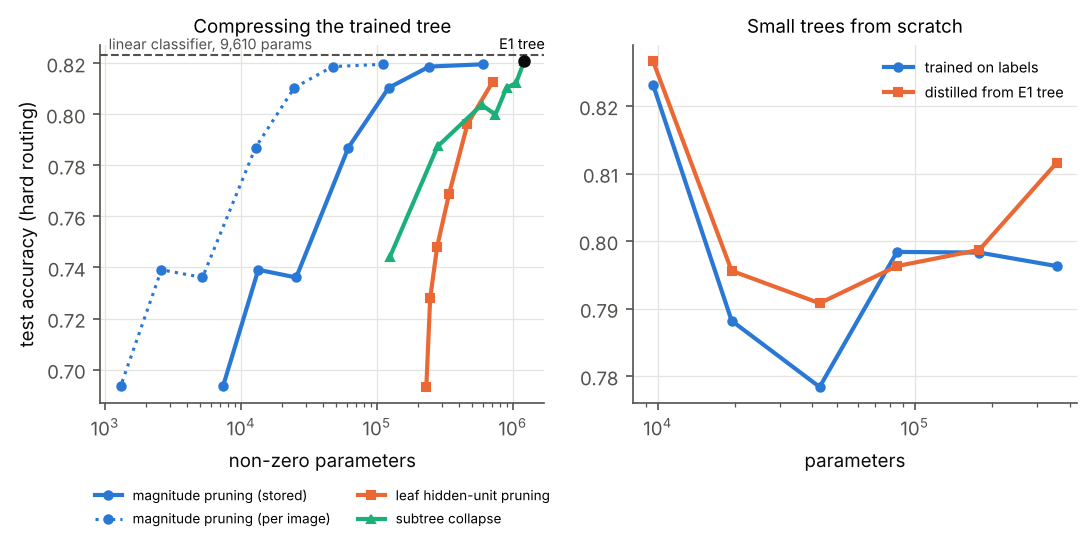
\includegraphics[width=\linewidth]{e4_cifar10.png}\\[2pt]
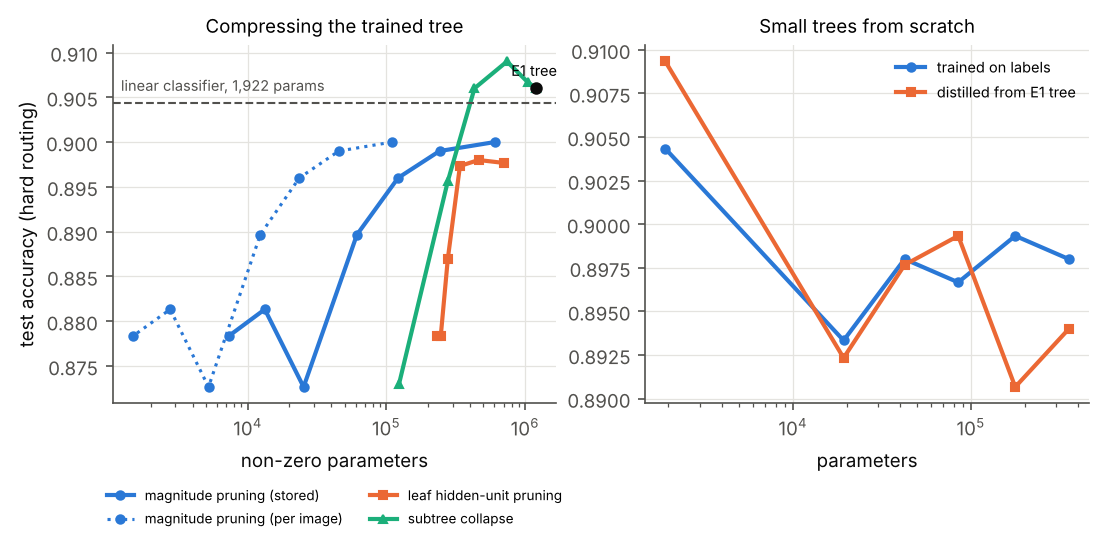
\includegraphics[width=\linewidth]{e4_catsdogs.png}
\caption{E4 on CIFAR-10 (top) and Cats vs Dogs (bottom). Left: compressing the E1 tree. Right: trees trained from scratch at each size; the leftmost point is a linear classifier (depth 0, no hidden layer).}
\label{fig:e4}
\end{figure}

The main result is the dashed line in Figure~\ref{fig:e4}: \textbf{a linear classifier on the same features, with 9.6k parameters on CIFAR-10 and 1.9k on Cats vs Dogs, is as accurate as the 1.2M-parameter tree} (82.3\% versus 82.5\%; 90.4\% versus 90.6\%), and a distilled linear classifier is slightly better than the tree it was distilled from (82.7\% and 90.9\%). The smallest network that matches the tree is therefore about 125 to 600 times smaller than it. The capacity of the big tree goes into memorising the training set, not into test accuracy.

The small trees trained from scratch (right panels) also show the smallest \emph{interpolating} tree. On CIFAR-10, a depth-2 tree with leaf width 16 (85k parameters) is the first to reach about 100\% training accuracy (99.95\%); smaller trees stop at 93.9\% and 98.2\%. Test accuracy goes from 82.3\% for the linear classifier down to 77.8\% at 43k parameters, where the tree can almost but not quite memorise the 45{,}000 images, and is back at 82.5\% for the 1.2M-parameter E1 tree. Cats vs Dogs shows the same dip, smaller (90.4\%, then 89.3\% at 19k, then 90.6\%). This is the double-descent shape on the full, clean training sets; Section~\ref{sec:dd} studies it under controlled conditions.

\section{E2: double descent}
\label{sec:dd}
\paragraph{Setup.} To see the whole curve, including the regime where the tree is too small to fit the data, the training set must be small relative to the largest tree. Every E2 run uses the first $n=2000$ CIFAR-10 (or Cats vs Dogs) training images, the ResNet-18 features projected onto their top 64 principal components (fitted on all training features, without labels), and a fraction of flipped labels (0\%, 10\% or 20\%). The tree has depth 2 (3 routers of width 4, 4 leaves) unless stated otherwise, and the leaf width $h$ is swept from 1 to 1024, which takes the tree from 1.1k to 308k parameters. Training is full-batch Adam for 4{,}000 steps with the squared loss, no weight decay and no early stopping. The test set is always the full, clean test set. Points are averages over 3 seeds (CIFAR-10, 0\% and 20\% noise), 2 seeds (Cats vs Dogs) or 1 seed (10\% noise and the largest width); shaded bands span the seeds.

\begin{figure}[!htbp]
\centering
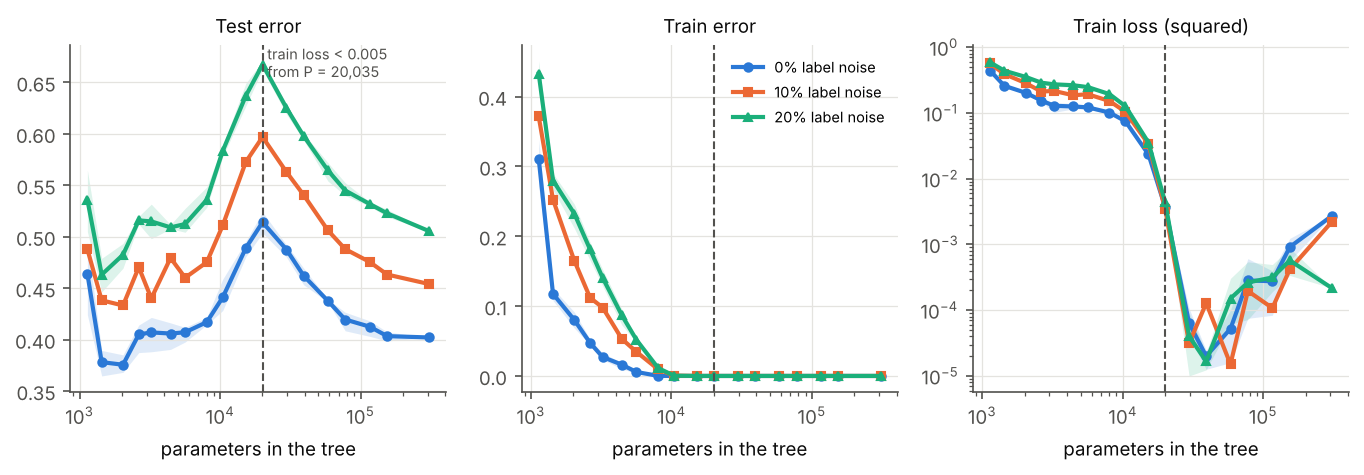
\includegraphics[width=\linewidth]{e2_width_cifar10.png}
\caption{CIFAR-10, model-wise double descent as the leaf width grows (depth 2, $n=2000$). Dashed line: the smallest tree whose final training loss is below 0.005. It coincides with $P=nK=20{,}000$. Training \emph{error} reaches 0 much earlier, at 8k to 10k parameters.}
\label{fig:width-c10}
\end{figure}

\paragraph{Model-wise double descent (Figure~\ref{fig:width-c10}).} On CIFAR-10 the test error follows the classical U-curve while the tree is small, then rises to a sharp peak where the training loss reaches zero, at $P\approx 20{,}000 = n\cdot K$ parameters (the number of numbers the tree has to fit), then falls again as the tree keeps growing:
\begin{center}\small
\begin{tabular}{lccc}
\toprule
label noise & best small tree & peak at $P\approx 20$k & largest tree (308k) \\
\midrule
0\% & 37.6\% (2.0k params) & 51.4\% & 40.2\% \\
10\% & 43.3\% (2.0k) & 59.7\% & 45.4\% \\
20\% & 46.3\% (1.4k) & 66.7\% & 50.5\% \\
\bottomrule
\end{tabular}
\end{center}
Label noise raises the peak (by 14, 16 and 20 points over the small-tree minimum) far more than it raises the rest of the curve, as reported for deep networks \cite{nakkiran2019}. The second descent is steep but, within the sizes we could afford, the largest tree does not beat the best small one on CIFAR-10.

\begin{figure}[!htbp]
\centering
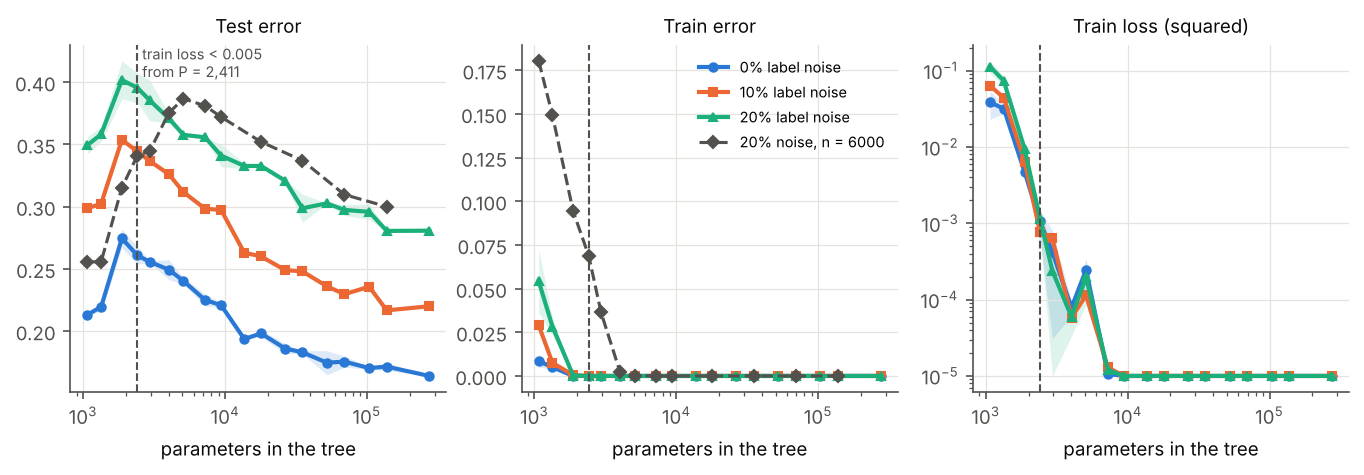
\includegraphics[width=\linewidth]{e2_width_catsdogs.png}
\caption{Cats vs Dogs, same setup ($K=2$). The peak is at about 2k parameters, where the training loss first drops below 0.005. Grey dashed: 20\% noise with $n=6000$ training images.}
\label{fig:width-cd}
\end{figure}

\paragraph{Cats vs Dogs (Figure~\ref{fig:width-cd}).} With two classes the tree reaches zero training loss already at about 2k parameters, so the first descent is short, but the peak and the long second descent are clear: test error goes from 21.3\% to a peak of 27.5\% and down to 16.4\% at 275k parameters (0\% noise), and from 34.9\% to 40.2\% and down to 28.1\% (20\% noise). Here the largest trees are the best. With three times as much data ($n=6000$, 20\% noise, grey curve) the peak moves right by about the same factor, to 5k--7k parameters (38.7\%); there, the smallest trees (25.6\%) beat every larger tree we trained.

\begin{figure}[!htbp]
\centering
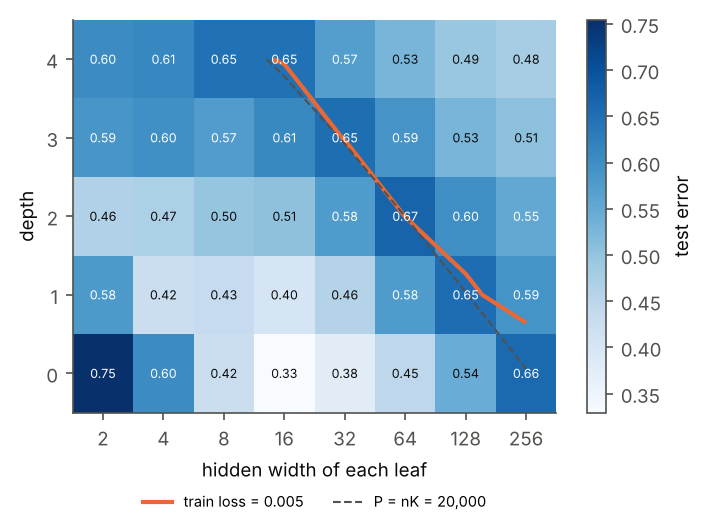
\includegraphics[width=0.62\linewidth]{e2_surface.png}
\caption{CIFAR-10, 20\% noise, test error over depth $\times$ leaf width (one seed). Orange: where the final training loss crosses 0.005. Dashed: trees with $P=20{,}000$ parameters. The worst cell of every row lies on these lines.}
\label{fig:surface}
\end{figure}

\paragraph{Width versus depth (Figure~\ref{fig:surface}).} A tree has two size knobs: how many leaves (depth) and how big each node is (width). We trained all 40 combinations of depth 0--4 and width 2--256. In every row, the worst test error (0.65 to 0.67) sits on the cell with $P\approx 14$k--23k parameters, and the interpolation contour and the line $P=nK$ run along the same diagonal of the grid. Whether parameters come from more leaves or wider leaves makes no difference to where the peak is: it is set by total size relative to $nK$. Adding leaves alone gives the same curve (Figure~\ref{fig:depth-samples}, left): with leaf width fixed at 16, test error goes from 33.2\% for a single network (depth 0, 1.2k parameters) up to 64.7\% at depth 4 (23k parameters, training loss $10^{-4}$) and back down to 48.6\% at depth 7 (189k parameters, 128 leaves).

\begin{figure}[!htbp]
\centering
\begin{minipage}{0.49\linewidth}\centering
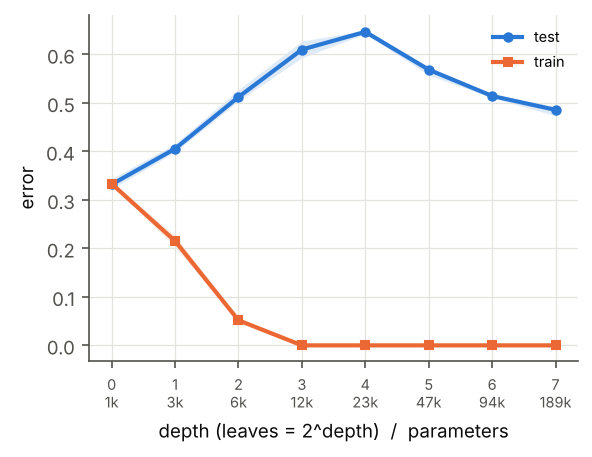
\includegraphics[width=\linewidth]{e2_depth.png}
\end{minipage}\hfill
\begin{minipage}{0.49\linewidth}\centering
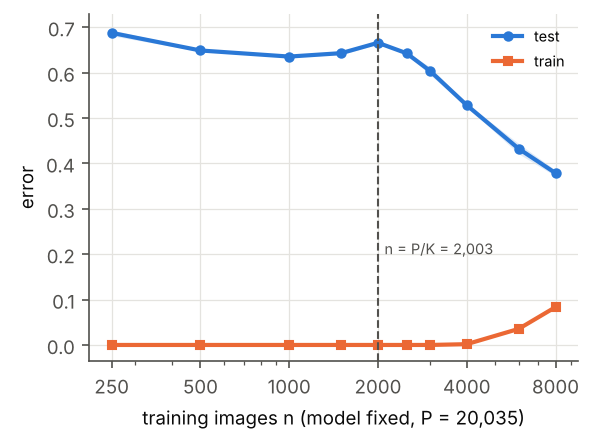
\includegraphics[width=\linewidth]{e2_samples.png}
\end{minipage}
\caption{Left: depth-wise sweep at leaf width 16 (20\% noise, 3 seeds); tick labels give depth and parameter count. Right: sample-wise sweep with the tree fixed at 20k parameters (20\% noise, 2 seeds).}
\label{fig:depth-samples}
\end{figure}

\paragraph{More data can hurt (Figure~\ref{fig:depth-samples}, right).} Holding the tree fixed at 20k parameters and growing the training set, test error first falls (68.7\% at $n=250$ to 63.5\% at $n=1000$), then rises to 66.6\% at $n=2000$, where $nK$ equals the parameter count, and only then falls steadily (37.8\% at $n=8000$). Doubling the data from 1000 to 2000 images makes this tree worse, because it moves the tree onto its interpolation point.

\begin{figure}[!htbp]
\centering
\begin{minipage}{0.49\linewidth}\centering
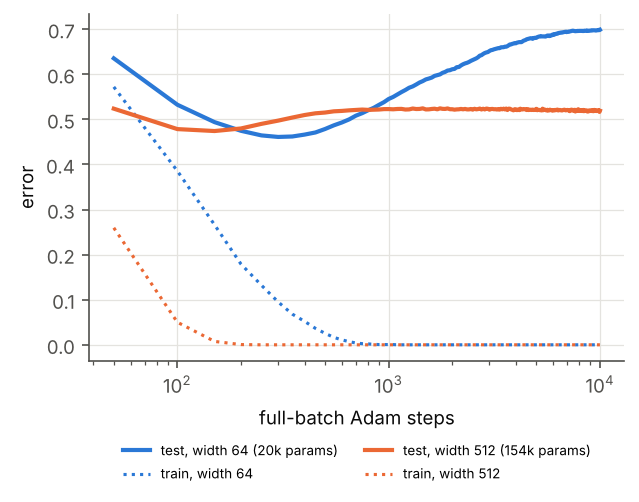
\includegraphics[width=\linewidth]{e2_epochs.png}
\end{minipage}\hfill
\begin{minipage}{0.49\linewidth}\centering
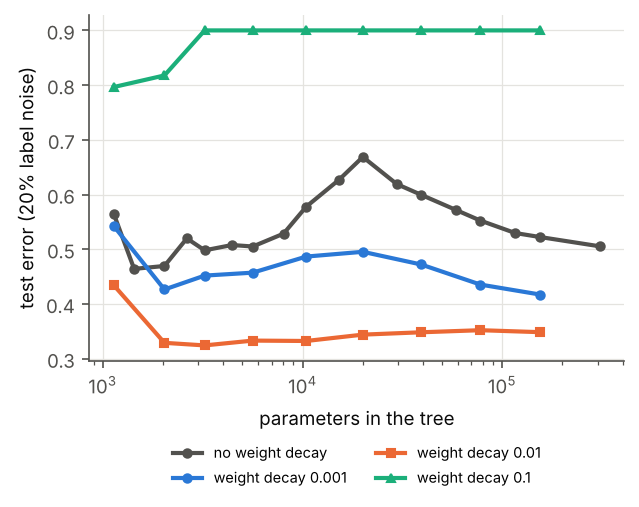
\includegraphics[width=\linewidth]{e2_wd.png}
\end{minipage}
\caption{Left: epoch-wise curves for a tree at the interpolation point (width 64) and well past it (width 512), 20\% noise. Right: the width sweep at 20\% noise with weight decay added (one seed).}
\label{fig:epochs-wd}
\end{figure}

\paragraph{Training time (Figure~\ref{fig:epochs-wd}, left).} We did \emph{not} see epoch-wise double descent. The tree at the interpolation point (width 64) reaches its best test error, 46.1\%, after 300 steps, while it still makes training errors; it then fits the flipped labels (zero training error from step 1{,}100) and its test error climbs to 66.9\% at step 4{,}000 and 69.9\% at step 10{,}000 as the training loss keeps shrinking. The wide tree (width 512) fits the training set by step 250, bottoms out at 47.4\%, and settles at 52\% with no further change. Two consequences: early stopping alone would erase the model-wise peak, and the height of the peak depends on how long training runs. Epoch-wise double descent in \cite{nakkiran2019} needed thousands of epochs of minibatch training on images; full-batch Adam on 64 fixed features may never enter the late regime where it appears.

\paragraph{Regularisation removes the peak (Figure~\ref{fig:epochs-wd}, right).} With weight decay $10^{-3}$ the peak at 20k parameters drops from 66.7\% to 49.5\%. With $10^{-2}$ there is no peak at all: test error stays between 32.4\% and 35.2\% for every width from 4 upwards (43.4\% at width 1), far better than any unregularised tree in the width sweep. These trees never drive the training loss to zero (it stays above 0.13), even at widths where they classify almost every training image as labelled. With $10^{-1}$ every tree collapses to a constant prediction (90\% error). This matches the result of Nakkiran et al.\ \cite{nakkiran2020} that well-tuned regularisation makes test error fall monotonically with size; double descent is a property of unregularised (or weakly regularised) training to zero loss.

\begin{figure}[!htbp]
\centering
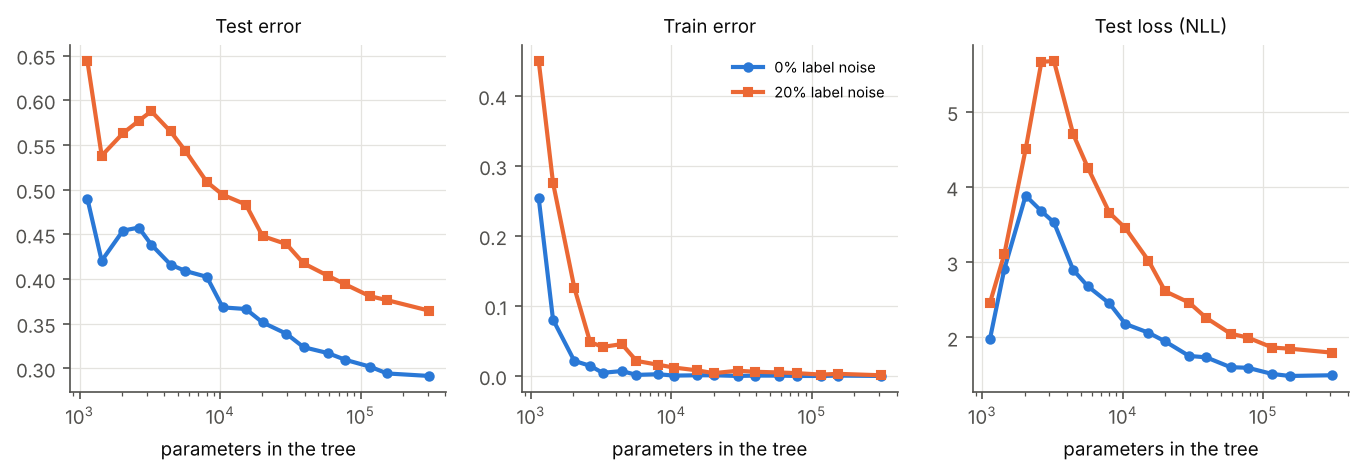
\includegraphics[width=\linewidth]{e2_width_cifar10_ce.png}
\caption{The CIFAR-10 width sweep with the mixture (cross-entropy) loss instead of the squared loss (one seed). The peak moves to about 3k parameters and is clearest in the test loss.}
\label{fig:ce}
\end{figure}

\paragraph{Cross-entropy (Figure~\ref{fig:ce}).} With the mixture loss the peak moves left, to 2.6k to 3.2k parameters, and is smaller in test error (from 42.0\% to 45.8\% with clean labels, from 53.8\% to 58.8\% with 20\% noise) but large in test loss. Past it, test error falls all the way to 29.4\% (clean) and 36.5\% (20\% noise) for the largest trees, much lower than with the squared loss. Cross-entropy only needs the correct class to win, so far fewer parameters suffice to fit every label, and the trees reach the second descent sooner.

\section{E5: where do the mislabelled images go?}
\label{sec:e5}
The double-descent peak is driven by label noise, so we followed the 400 mislabelled images (20\% of $n=2000$) through trees below, at and above the interpolation point (same setup as E2; depth 2 with widths 4 to 1024, and depth 4 with widths 1 to 64). Three questions:
\begin{enumerate}
\item \emph{Do the routers isolate them?} Before running this, we expected the tree to \emph{quarantine} mislabelled images in a few small leaves, leaving the other leaves clean. We measured each leaf's share of mislabelled images under hard routing.
\item \emph{Do the routers bend to the wrong label?} For each class we know which leaves its correctly labelled images go to. A mislabelled image is \emph{label-routed} if its leaf is more typical of its (wrong) given label than of its true class. As a control, the same test is applied to clean images with a random fake label.
\item \emph{How far does the damage spread?} For each test image we find its nearest training image (in the 64-dimensional feature space). When that neighbour is mislabelled, how often does the tree predict the neighbour's wrong label, and how much higher is the test error there than near clean neighbours?
\end{enumerate}

\begin{table}[!htbp]
\centering\footnotesize
\begin{tabular}{rrrrrrrr}
\toprule
depth & width & params & test err & copies noisy NN label & err, NN noisy & err, NN clean & label-routed (control) \\
\midrule
2 & 4 & 2.0k & 46.9 & 8.5 & 50.7 & 46.1 & 42.0 (30.7) \\
2 & 16 & 5.6k & 50.5 & 9.6 & 55.0 & 49.5 & 53.7 (39.2) \\
2 & 64 & 20k & 66.9 & 14.6 & 73.8 & 65.2 & 47.0 (40.9) \\
2 & 256 & 78k & 55.2 & 15.9 & 63.8 & 53.2 & 47.3 (41.7) \\
2 & 1024 & 308k & 50.5 & 16.3 & 59.0 & 48.5 & 43.0 (43.6) \\
4 & 1 & 5.3k & 61.1 & 10.8 & 66.3 & 59.9 & 52.5 (29.7) \\
4 & 4 & 8.9k & 61.2 & 11.9 & 64.6 & 60.4 & 42.5 (32.4) \\
4 & 16 & 23k & 64.8 & 13.2 & 69.0 & 63.8 & 46.5 (33.5) \\
4 & 64 & 81k & 52.8 & 15.0 & 59.1 & 51.4 & 48.2 (36.2) \\
\bottomrule
\end{tabular}

\caption{E5 on CIFAR-10, 20\% noise. ``copies noisy NN label'': share of test images whose nearest training image is mislabelled and which receive that wrong label. ``err, NN noisy/clean'': test error on test images whose nearest training image is mislabelled / correctly labelled (19\% / 81\% of the test set). Label-routed: share of mislabelled training images whose leaf is more typical of the wrong label; the control is the same statistic for clean images with a random fake label.}
\label{tab:e5}
\end{table}

\begin{figure}[!htbp]
\centering
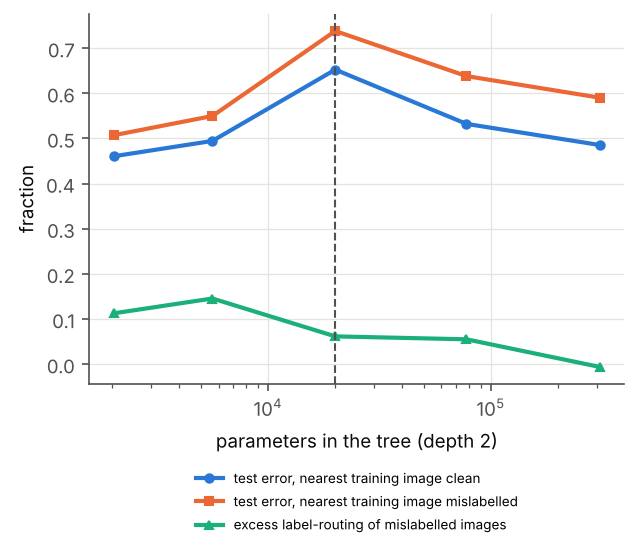
\includegraphics[width=0.55\linewidth]{e5_noise.png}
\caption{E5, depth-2 trees, 20\% noise. Dashed: the interpolation point. Excess label-routing is the label-routed share minus its control.}
\label{fig:e5}
\end{figure}

\paragraph{No quarantine.} The hypothesis was wrong. No leaf in any tree has twice the overall noise rate. Per-leaf noise rates lie between 14\% and 31\% in the depth-4 tree with width 64; the spread is widest in the smallest tree (depth 4, one hidden unit per leaf), whose two smallest leaves (16 and 19 images) have noise rates near 38\%. Mislabelled images are spread across all leaves, and each leaf memorises its own share.

\paragraph{Small leaves make the routers memorise.} Mislabelled images are label-routed more often than the control in every tree except the largest (Table~\ref{tab:e5}). The excess is largest when the leaves are too small to memorise anything themselves: 23 points for depth 4 with width 1 and 15 points for depth 2 with width 16. For depth 2 it falls to 6 points at and past the interpolation point and to zero at width 1024; with 16 leaves (depth 4) it stays at 10 to 13 points up to width 64. When the leaves can only draw simple boundaries, the routers absorb the wrong labels by steering mislabelled images to the leaves where images of the wrong class usually go. When the leaves are large, the leaves absorb them and the routing stays based on appearance.

\paragraph{The damage becomes local.} As the tree grows, it copies the wrong label of a mislabelled neighbour more often (8.5\% at width 4, 16.3\% at width 1024), and the error gap between test images near mislabelled and near clean training images widens from 4.6 to 10.5 points. Yet test error near \emph{clean} training images falls from 65.2\% at the interpolation point to 48.5\% at width 1024. The second descent therefore comes from test images away from the mislabelled ones. This is consistent with the large tree fitting each wrong label locally and staying smooth elsewhere, while the tree at the interpolation point distorts its function over a wider region to fit them. This matches the ``spiked-smooth'' picture of interpolating classifiers \cite{wyner2017}, and the tree adds a detail to it: which part of the tree does the fitting (routers or leaves) depends on leaf size.

\section{Interpretation}
\label{sec:interp}
\paragraph{Where the capacity goes.} On these datasets a tree of small networks can always be made to fit every training label, including deliberately wrong ones, and doing so is cheap: ten trees of 0.3M to 1.3M parameters reached 100\% training accuracy in at most 125 epochs on a CPU. What the tree does with that capacity depends on the regime. Below the interpolation point the tree cannot fit everything and test error follows the classical U-curve. At the interpolation point the tree has just enough parameters to fit all $nK$ targets, so the fit is forced through every mislabelled or atypical image with large weights and sharp bends, and test error peaks. Past it, many functions fit the data, and training from a small initialisation tends to reach a smoother one, so test error falls again. This is the standard account of double descent \cite{belkin2019, nakkiran2019}, and the tree follows it closely. With the squared loss, the peak sits at $P\approx nK$ whether the parameters are added by widening the leaves or by adding leaves (Figure~\ref{fig:surface}). For trees, the second descent here is a property of total size and not an artefact of switching from one complexity axis to another, which is how Curth et al.\ \cite{curth2023} explained the double descent of random forests and boosting.

\paragraph{The loss sets the threshold.} With cross-entropy the peak is at about 3k parameters instead of 20k (Figure~\ref{fig:ce}). Cross-entropy only needs the right class to have the highest score, which takes far fewer parameters than reproducing $nK$ one-hot numbers. ``Interpolation'' has to be defined by the loss being minimised, not by training accuracy: the squared-loss trees reach 0\% training error at 8k to 10k parameters, well before the peak at 20k.

\paragraph{Routing is not classification.} A tree is often pictured as splitting classes into ever finer groups. The receptive-field analysis shows that this happens only partly on CIFAR-10 and not at all on Cats vs Dogs, where the routers sort images by background, colour and framing and every leaf is a cat-versus-dog expert for one kind of photograph. Routers follow the largest variations in their input features, and the class is only one of them. Which variations a router can see is fixed by the trunk: a task-trained CNN gives object-centred, part-like routers; a frozen ImageNet ResNet gives scene-level ones.

\paragraph{The tree is much larger than it needs to be.} On frozen features, the 1.2M-parameter tree and a linear classifier with 125 to 600 times fewer parameters have the same test accuracy, and a distilled linear classifier is slightly better. The extra parameters are spent on memorising the training set, which the double-descent experiments show is harmless only once the tree is far past the interpolation point. For deployment, hard routing plus magnitude pruning gives a tree that runs 2.6k to 25k weights per image. A larger gain from a tree would come from conditional computation in the trunk itself, which these experiments do not test.

\section{Limitations}
\begin{itemize}
\item The class notes defining the course's tree network were not available to us; the model here is the standard soft decision tree / hierarchical mixture of experts with neural nodes, and the hard tree is its zero-temperature limit.
\item Everything ran on 2 CPU cores. The double-descent sweeps therefore use 2{,}000 training images and 64 PCA dimensions of the ResNet features, 1 to 3 seeds per point, and a fixed budget of 4{,}000 full-batch steps. Near the interpolation point training converges slowly, so part of the peak height can come from incomplete optimisation; the training-loss panels show how close each run got.
\item The trunks are frozen. Training trunk and tree together, as in Adaptive Neural Trees \cite{tanno2019}, could change both accuracy and routing.
\item Input-gradient saliency is a noisy explanation method \cite{adebayo2018}; we use it only for coarse statistics (how central, how spread) and for comparisons between trunks, and back it with prototypes and class statistics.
\end{itemize}

\section{Future directions}
\begin{itemize}
\item \emph{Train the trunk with the tree.} Put a small convolutional block on each edge (Adaptive Neural Trees) so that each branch learns its own features, and test whether the receptive fields then shrink with depth.
\item \emph{Use routing to find shortcuts.} The Cats vs Dogs routers isolate backgrounds and settings. Evaluating each leaf on images with swapped backgrounds would measure how much each expert depends on context.
\item \emph{Effective parameters for trees.} Measure the generalised effective number of parameters of Curth et al.\ for neural trees and check whether the 2-D surface folds into a single U-curve when plotted against it.
\item \emph{Grow and prune with validation.} Replace the fixed depth with greedy growth (split or deepen a leaf only if validation loss drops) and the greedy collapse of E4, giving a tree whose size is chosen by the data.
\item \emph{Complexity penalties at the nodes.} Add a VC-dimension-based penalty \cite{jayadeva2017} to each router and leaf, and compare the resulting sizes with magnitude pruning.
\item \emph{Regression.} The squared-loss tree used in E2 is already a regression tree on one-hot targets; running it on real regression data would test whether the same double-descent surface appears.
\end{itemize}

\section{Code and reproduction}
The repository (\repo) is organised as follows; the README gives the exact commands.
\begin{center}\small
\begin{tabular}{ll}
\toprule
\texttt{treenet/data.py} & download format, fixed splits, label noise \\
\texttt{treenet/features.py} & the three trunks and feature caching \\
\texttt{treenet/tree.py} & \texttt{SoftTree}, losses, balance penalty, hard routing \\
\texttt{treenet/train.py} & training loop and evaluation \\
\texttt{experiments/e1\_overfit.py} & E1 (Table~\ref{tab:e1}) \\
\texttt{experiments/e2\_double\_descent.py}, \texttt{run\_e2.sh} & E2 sweeps (Section~\ref{sec:dd}) \\
\texttt{experiments/e3\_receptive\_fields.py} & E3 (Section~\ref{sec:rf}) \\
\texttt{experiments/e4\_compress.py} & E4 (Section~\ref{sec:e4}) \\
\texttt{experiments/e5\_noise.py} & E5 (Section~\ref{sec:e5}) \\
\texttt{experiments/make\_figures.py}, \texttt{make\_tables.py} & every figure and table in this report \\
\bottomrule
\end{tabular}
\end{center}
Raw results (one JSON line per trained model, with training curves) are in \texttt{results/}. Total compute for everything in this report was about 6 hours on 2 CPU cores.

\begin{thebibliography}{99}\small
\bibitem{adebayo2018} J.~Adebayo, J.~Gilmer, M.~Muelly, I.~Goodfellow, M.~Hardt, B.~Kim. Sanity checks for saliency maps. \emph{NeurIPS}, 2018.
\bibitem{belkin2019} M.~Belkin, D.~Hsu, S.~Ma, S.~Mandal. Reconciling modern machine-learning practice and the classical bias--variance trade-off. \emph{PNAS} 116(32), 2019.
\bibitem{curth2023} A.~Curth, A.~Jeffares, M.~van~der~Schaar. A U-turn on double descent: rethinking parameter counting in statistical learning. \emph{NeurIPS}, 2023.
\bibitem{frosst2017} N.~Frosst, G.~Hinton. Distilling a neural network into a soft decision tree. arXiv:1711.09784, 2017.
\bibitem{he2016} K.~He, X.~Zhang, S.~Ren, J.~Sun. Deep residual learning for image recognition. \emph{CVPR}, 2016.
\bibitem{jayadeva2017} Jayadeva, H.~Pant, M.~Sharma, A.~Dubey, S.~Soman, S.~Tripathi, S.~Guruju, N.~Goalla. Learning neural network classifiers with low model complexity. arXiv:1707.09933, 2017.
\bibitem{jordan1994} M.~I.~Jordan, R.~A.~Jacobs. Hierarchical mixtures of experts and the EM algorithm. \emph{Neural Computation} 6(2), 1994.
\bibitem{luo2016} W.~Luo, Y.~Li, R.~Urtasun, R.~Zemel. Understanding the effective receptive field in deep convolutional neural networks. \emph{NeurIPS}, 2016.
\bibitem{nakkiran2019} P.~Nakkiran, G.~Kaplun, Y.~Bansal, T.~Yang, B.~Barak, I.~Sutskever. Deep double descent: where bigger models and more data hurt. \emph{ICLR}, 2020 (arXiv:1912.02292).
\bibitem{nakkiran2020} P.~Nakkiran, P.~Venkat, S.~Kakade, T.~Ma. Optimal regularization can mitigate double descent. \emph{ICLR}, 2021.
\bibitem{tanno2019} R.~Tanno, K.~Arulkumaran, D.~Alexander, A.~Criminisi, A.~Nori. Adaptive neural trees. \emph{ICML}, 2019.
\bibitem{wyner2017} A.~J.~Wyner, M.~Olson, J.~Bleich, D.~Mease. Explaining the success of AdaBoost and random forests as interpolating classifiers. \emph{JMLR} 18(48), 2017.
\end{thebibliography}


\end{document}
